\section{LTasks}\label{section-ltasks}
To continue the naming scheme of iTasks and mTasks, the proof of concept implementation in this thesis is called LTasks\footnote{With capital ``L'' to avoid confusion with iTasks, because many fonts make the lowercase ``l'' look like a capital ``I''.}. This section goes into the details of the LTasks library and shows that it is indeed a correct implementation of TOP. To further show that the proof of concept is indeed complete for TOP, chapter \ref{comparison} contains a case study comparison of the breakfast example, while appendix \ref{appendix-examples} contains full examples in both LTasks and iTasks. The full code is available at \url{https://github.com/Dantevg/LTasks}, the files \lua{task.lua}, \lua{types.lua} and \lua{ltuiEditor.lua} are attached in appendix \ref{appendix-ltask}.

\subsection{Tasks}
Most functions in the LTask library are defined in the \lua{task} module (\ref{appendix-ltask-task.lua}), as functions on the \lua{task} table. The function \lua{task.new} (listing \ref{lst:ltasks_task.new}) creates a task, which is a table containing the task coroutine, the task value and its stability. The metatable of the task has a \lua{__index} field pointing to the \lua{task} table, so all operations can be done as methods on a task, and chained. The metatable also defines the custom operator behaviour (\ref{section-ltasks-combinators}, listing \ref{lst:ltasks_operators_definition}).

The function \lua{task.resume} (listing \ref{lst:ltasks_task.resume}) is for resuming a task's coroutine. When calling this function, you can give it a table of options used for the user interface: the boolean \lua{showUI} and the task \lua{parent}. The options will be explained further in section \ref{section-ltasks-ltui}. When a task is resumed, it can resume any child tasks it has. When it is done, it yields. This creates a coroutine hierarchy.

\RecustomVerbatimEnvironment{Verbatim}{Verbatim}{} % enable line numbers

\begin{figure}[ht]
\centering
\inputminted[linenos, firstline=12, lastline=19]{lua}{code/task.lua}
\vspace{-\baselineskip}
\caption{The \lua{task.new} function.}
\label{lst:ltasks_task.new}
\end{figure}

\begin{figure}[ht]
\centering
\inputminted[linenos, firstline=310, lastline=327]{lua}{code/task.lua}
\vspace{-\baselineskip}
\caption{The \lua{task.resume} function for resuming a task's coroutine.}
\label{lst:ltasks_task.resume}
\end{figure}

\begin{figure}[ht]
\centering
\begin{minted}[linenos, firstnumber=337]{lua}
task.__band = task.parallelAnd
task.__bor = task.parallelOr
task.__bxor = task.step
task.__concat = task.step
\end{minted}
\vspace{-\baselineskip}
\caption{Setting the custom operator behaviour to functions defined in the \lua{task} table.}
\label{lst:ltasks_operators_definition}
\end{figure}

\subsection{Task combinators}\label{section-ltasks-combinators}
While iTasks provides a lot of combinators, we do not need that for a proof of concept so LTasks includes only the essential combinators and some convenience wrappers around them. Here is the list, along with their operators in LTasks or their equivalent in iTasks:
\begin{itemize}
    \item \lua{constant} (\clean{return} in iTasks)
    \item \lua{step} (\lua{~} in LTasks, \clean{>>*} in iTasks), \lua{stepStable} (\clean{>>-} in iTasks) and \linebreak \lua{stepButtonStable} (\clean{>>?} in iTasks)
    \item \lua{parallel}, \lua{anyTask}, \lua{parallelAnd} (\lua{&} in LTasks, \clean{-&&-} in iTasks), \lua{parallelOr} (\lua{|} in LTasks, \clean{-||-} in iTasks), \lua{parallelLeft} (\clean{-||} in iTasks) and \lua{parallelRight} (\clean{||-} in iTasks)
    \item \lua{transform} and \lua{transformValue} (\clean{@} in iTasks)
\end{itemize}

These are the most important functions for building a TOP system, as we defined at the start of this chapter.

\subsubsection{Step}
The step combinator in LTasks implements both \clean{OnValue} and \clean{OnAction}. When there are multiple continuations that run on the same action, the UI shows the user a dialog to choose one of the continuations to step to. iTasks does not handle this well, due to what is probably a bug: it displays two buttons with the same name, but chooses the first task continuation regardless of which button is pressed. For this reason we used two different actions in listing \ref{lst:clean_step_onaction}.

In the example in listing \ref{lst:ltasks_step}, this happens when the user inputs ``Madam, I'm Adam''---which is both a palindrome and a greeting. LTasks will prompt the user which continuation to step to.

\RecustomVerbatimEnvironment{Verbatim}{BVerbatim}{} % reset line numbers

\begin{figure}
\centering
\begin{minted}{lua}
editor.editString("") ~ {
    {
        action = "continue",
        fn = function(value)
            return isPalindrome(value)
                and editor.viewInformation(value, "palindrome: ")
        end
    }, {
        action = "continue",
        fn = function(value)
            return isGreeting(value)
                and editor.viewInformation(value, "greeting: ")
        end
    }
}
\end{minted}
\caption{The step combinator in LTasks, using multiple \clean{OnAction} continuations of the same action. Listing \ref{lst:clean_step_onaction} shows this example in iTasks.}
\label{lst:ltasks_step}
\end{figure}

The implementation of \lua{step} can be divided into three phases: before the step happens, choosing the continuation task, and after the step happens.
Before the step happens, each time the \lua{step} task is resumed, it resumes its first task and searches for a matching continuation task (listing \ref{lst:ltasks_task.step_1}). For that matching, it uses the function \lua{matchContinuation}, which finds all continuations that have the right type and action, and have a type that is as specific as the most specific continuation.
If it has found at least one continuation, it goes on to the continuation choosing phase. If there are multiple continuation tasks that match, it lets the user choose which one to step to (listing \ref{lst:ltasks_task.step_2}).
When it has a single continuation task, it steps to that task and acts like a proxy: it sets its own value and stability to that of the continuation task (listing \ref{lst:ltasks_task.step_3}).

\RecustomVerbatimEnvironment{Verbatim}{Verbatim}{} % enable line numbers

\begin{figure}
\centering
\inputminted[linenos, firstline=93, lastline=106]{lua}{code/task.lua}
\vspace{-\baselineskip}
\caption{The first phase of the \lua{task.step} function, before the step happens.}
\label{lst:ltasks_task.step_1}
\end{figure}

\begin{figure}
\centering
\inputminted[linenos, firstline=108, lastline=122]{lua}{code/task.lua}
\vspace{-\baselineskip}
\caption{The continuation selection phase of the \lua{task.step} function, asking the user which continuation task to step to.}
\label{lst:ltasks_task.step_2}
\end{figure}

\begin{figure}
\centering
\inputminted[linenos, firstline=124, lastline=133]{lua}{code/task.lua}
\vspace{-\baselineskip}
\caption{The last phase of the \lua{task.step} function, after the step happens.}
\label{lst:ltasks_task.step_3}
\end{figure}

\RecustomVerbatimEnvironment{Verbatim}{BVerbatim}{} % reset line numbers

\subsubsection{Parallel}
The parallel task combinator in LTasks is a simplified version of the one in iTasks, but the most common usage is present: combining tasks into a list of task values. Listing \ref{lst:ltasks_parallel} shows a simple example of this.

\begin{figure}
\centering
\begin{minted}{lua}
(task.constant "A" & task.constant "B") ~ {{
    fn = function(x) return editor.viewInformation(x) end
}}
\end{minted}
\caption{The parallel combinator in LTasks. The output of this is \lua{{"A", "B"}}. Listing \ref{lst:clean_parallel} shows this example in iTasks.}
\label{lst:ltasks_parallel}
\end{figure}

Listing \ref{lst:ltasks_task.parallel} shows the most important part of the \lua{task.parallel} function. Each time it is resumed, it resumes all of its child tasks and updates its own value to be the list of values and stabilities of the child tasks. It is itself stable if all child tasks are stable.

\begin{figure}
\centering
\RecustomVerbatimEnvironment{Verbatim}{Verbatim}{} % enable line numbers
\inputminted[linenos, firstline=218, lastline=231]{lua}{code/task.lua}
\RecustomVerbatimEnvironment{Verbatim}{BVerbatim}{} % reset line numbers
\vspace{-\baselineskip}
\caption{The content of the \lua{task.parallel} task.}
\label{lst:ltasks_task.parallel}
\end{figure}

\subsubsection{Custom operators}
In Clean it is common to define lots of operators. For example, there are eight different operators for variations of the step combinator. Lua does allow for changing the behaviour of the standard operators, but only up to a point. For example, the result of the comparison operators like \lua{<} is always converted to a boolean \cite{luareferencemanual}. Perhaps the most notable library that uses operators with custom behaviour is LPeg\footnote{\url{http://www.inf.puc-rio.br/~roberto/lpeg/}}. It is not so common to redefine the behaviour of the operators in Lua, so LTasks only uses three operators: \lua{~}, \lua{&} and \lua{|}. Using the \lua{..} operator for \lua{step} more resembles the original meaning---concatenation, putting strings after each other. However that operator does not play well with chaining multiple operators because it is right-associative \cite[\S 3.4.8]{luareferencemanual}.

\subsection{Type matching}
For time reasons, we did not implement a custom type matching algorithm (one that matches the empty table \lua{{}} for the type \lua{"table"} for example). We just used the Typed\footref{footnote-typed} library to compare types, which is very strict in what it matches. There is a Lua library for matching data structures called Tamale\footnote{\url{https://luarocks.org/modules/luarocks/tamale}}, however it is not made for matching types and is also strict in what it matches, so we do not use it.

We did implement the type \textit{specificity} algorithm for ordering types from section \ref{section-combinators-type-matching}. The function \lua{types.lt} in module \lua{types.lua} (\ref{appendix-ltask-types.lua}, lines 63--136) follows these rules, and returns \lua{true} when a type is less specific than another. It parses the types the same way as the Typed library\footref{footnote-typed}. This is important, because Typed itself is first used to check whether a type is even compatible. We do not check for list length, because the Typed library does not allow specifying that. This type specificity algorithm can be seen in action for example when there are two continuation tasks, one of which accepts \lua{"string"} and the other accepts \lua{"string | number"}. When a string value is given, the first continuation task is chosen, even though the second one also matches.

\subsection{Editors}
Instead of providing a single function for creating all types of user input editors like iTasks does, we provide one function per editor type: \lua{editNumber}, \lua{editTable} etc. To create a table editor, the programmer has to provide the table editor with the sub-editors. Listing \ref{lst:ltasks_editors_table} shows what this looks like.

Each editor construction function has an optional parameter for setting the editor's prompt (called a hint in iTasks). This is done to keep the proof-of-concept simple: iTasks uses a \clean{tune} combinator (with \clean{<<@} operator) which can do a lot more, but that is not important for TOP.

\begin{figure}[ht]
\centering
\begin{minted}{lua}
local dateEditor = editor.editTable {
    year = editor.editNumber(),
    month = editor.editString(),
    day = editor.editNumber(),
}
\end{minted}
\caption{Creating a table editor with three sub-editors for \lua{year}, \lua{month} and \lua{day} (adapted from the date example in appendix \ref{appendix-dates}).}
\label{lst:ltasks_editors_table}
\end{figure}

\subsection{User Interface with LTUI}\label{section-ltasks-ltui}
For simplicity with working with LTUI, we decided to only ever have one UI element of a type at once. Instead of creating a new element every time, the old one is re-used, displayed, and hidden when no longer needed. These re-used elements are defined and created once in \lua{ltuiApp.lua}.
The module \lua{ltuiElements.lua} provides functions that use these reusable elements and set the contents like the task name or the current value.
\lua{ltuiEditor.lua} is the module that then converts these editors into tasks so they can be used with TOP. This module provides the same functions with the same parameters as \lua{terminalEditor.lua}, which provides editors that use standard I/O as a command-line interface instead of a textual UI. Figure \ref{fig:comparison_ltask_ui} shows the textual user interface in action.

When resuming a task's coroutine, you can pass it options related to the user interface. The boolean \lua{showUI} is read by tasks that have a visible UI (so editors and \lua{step}, but not \lua{transform}). When resuming any child tasks, they set this to \lua{false}. The task \lua{parent} is passed by tasks that have a visible UI to their child tasks. When a task exits its UI (by selecting ``back'' or when an editor dialog closes), it resumes its parent task with \lua{showUI} enabled, in order for it to update its visible content.

To create a TOP application with a LTUI user interface, \lua{ltuiApp.lua} first creates a \lua{ltui.application}. The main entry point for the application, \lua{ltuiTest.lua}, expands on this by defining \lua{app.init} and \lua{app.on_refresh} functions. LTUI calls the \lua{app.on_refresh} function multiple times per second, which first resumes the top-level task, and then lets LTUI handle any events and draw the UI.

\begin{figure}
\centering
\RecustomVerbatimEnvironment{Verbatim}{Verbatim}{} % enable line numbers
\begin{minted}{lua}
function app:on_refresh()
	if self.task then self.task:resume() end
	
	ltui.application.on_refresh(self)
end
\end{minted}
\RecustomVerbatimEnvironment{Verbatim}{BVerbatim}{} % reset line numbers
\vspace{-\baselineskip}
\caption{The \lua{app.on_refresh} function.}
\label{lst:ltasks_ltuiTest.on_refresh}
\end{figure}

% \begin{figure}
%     \centering
%     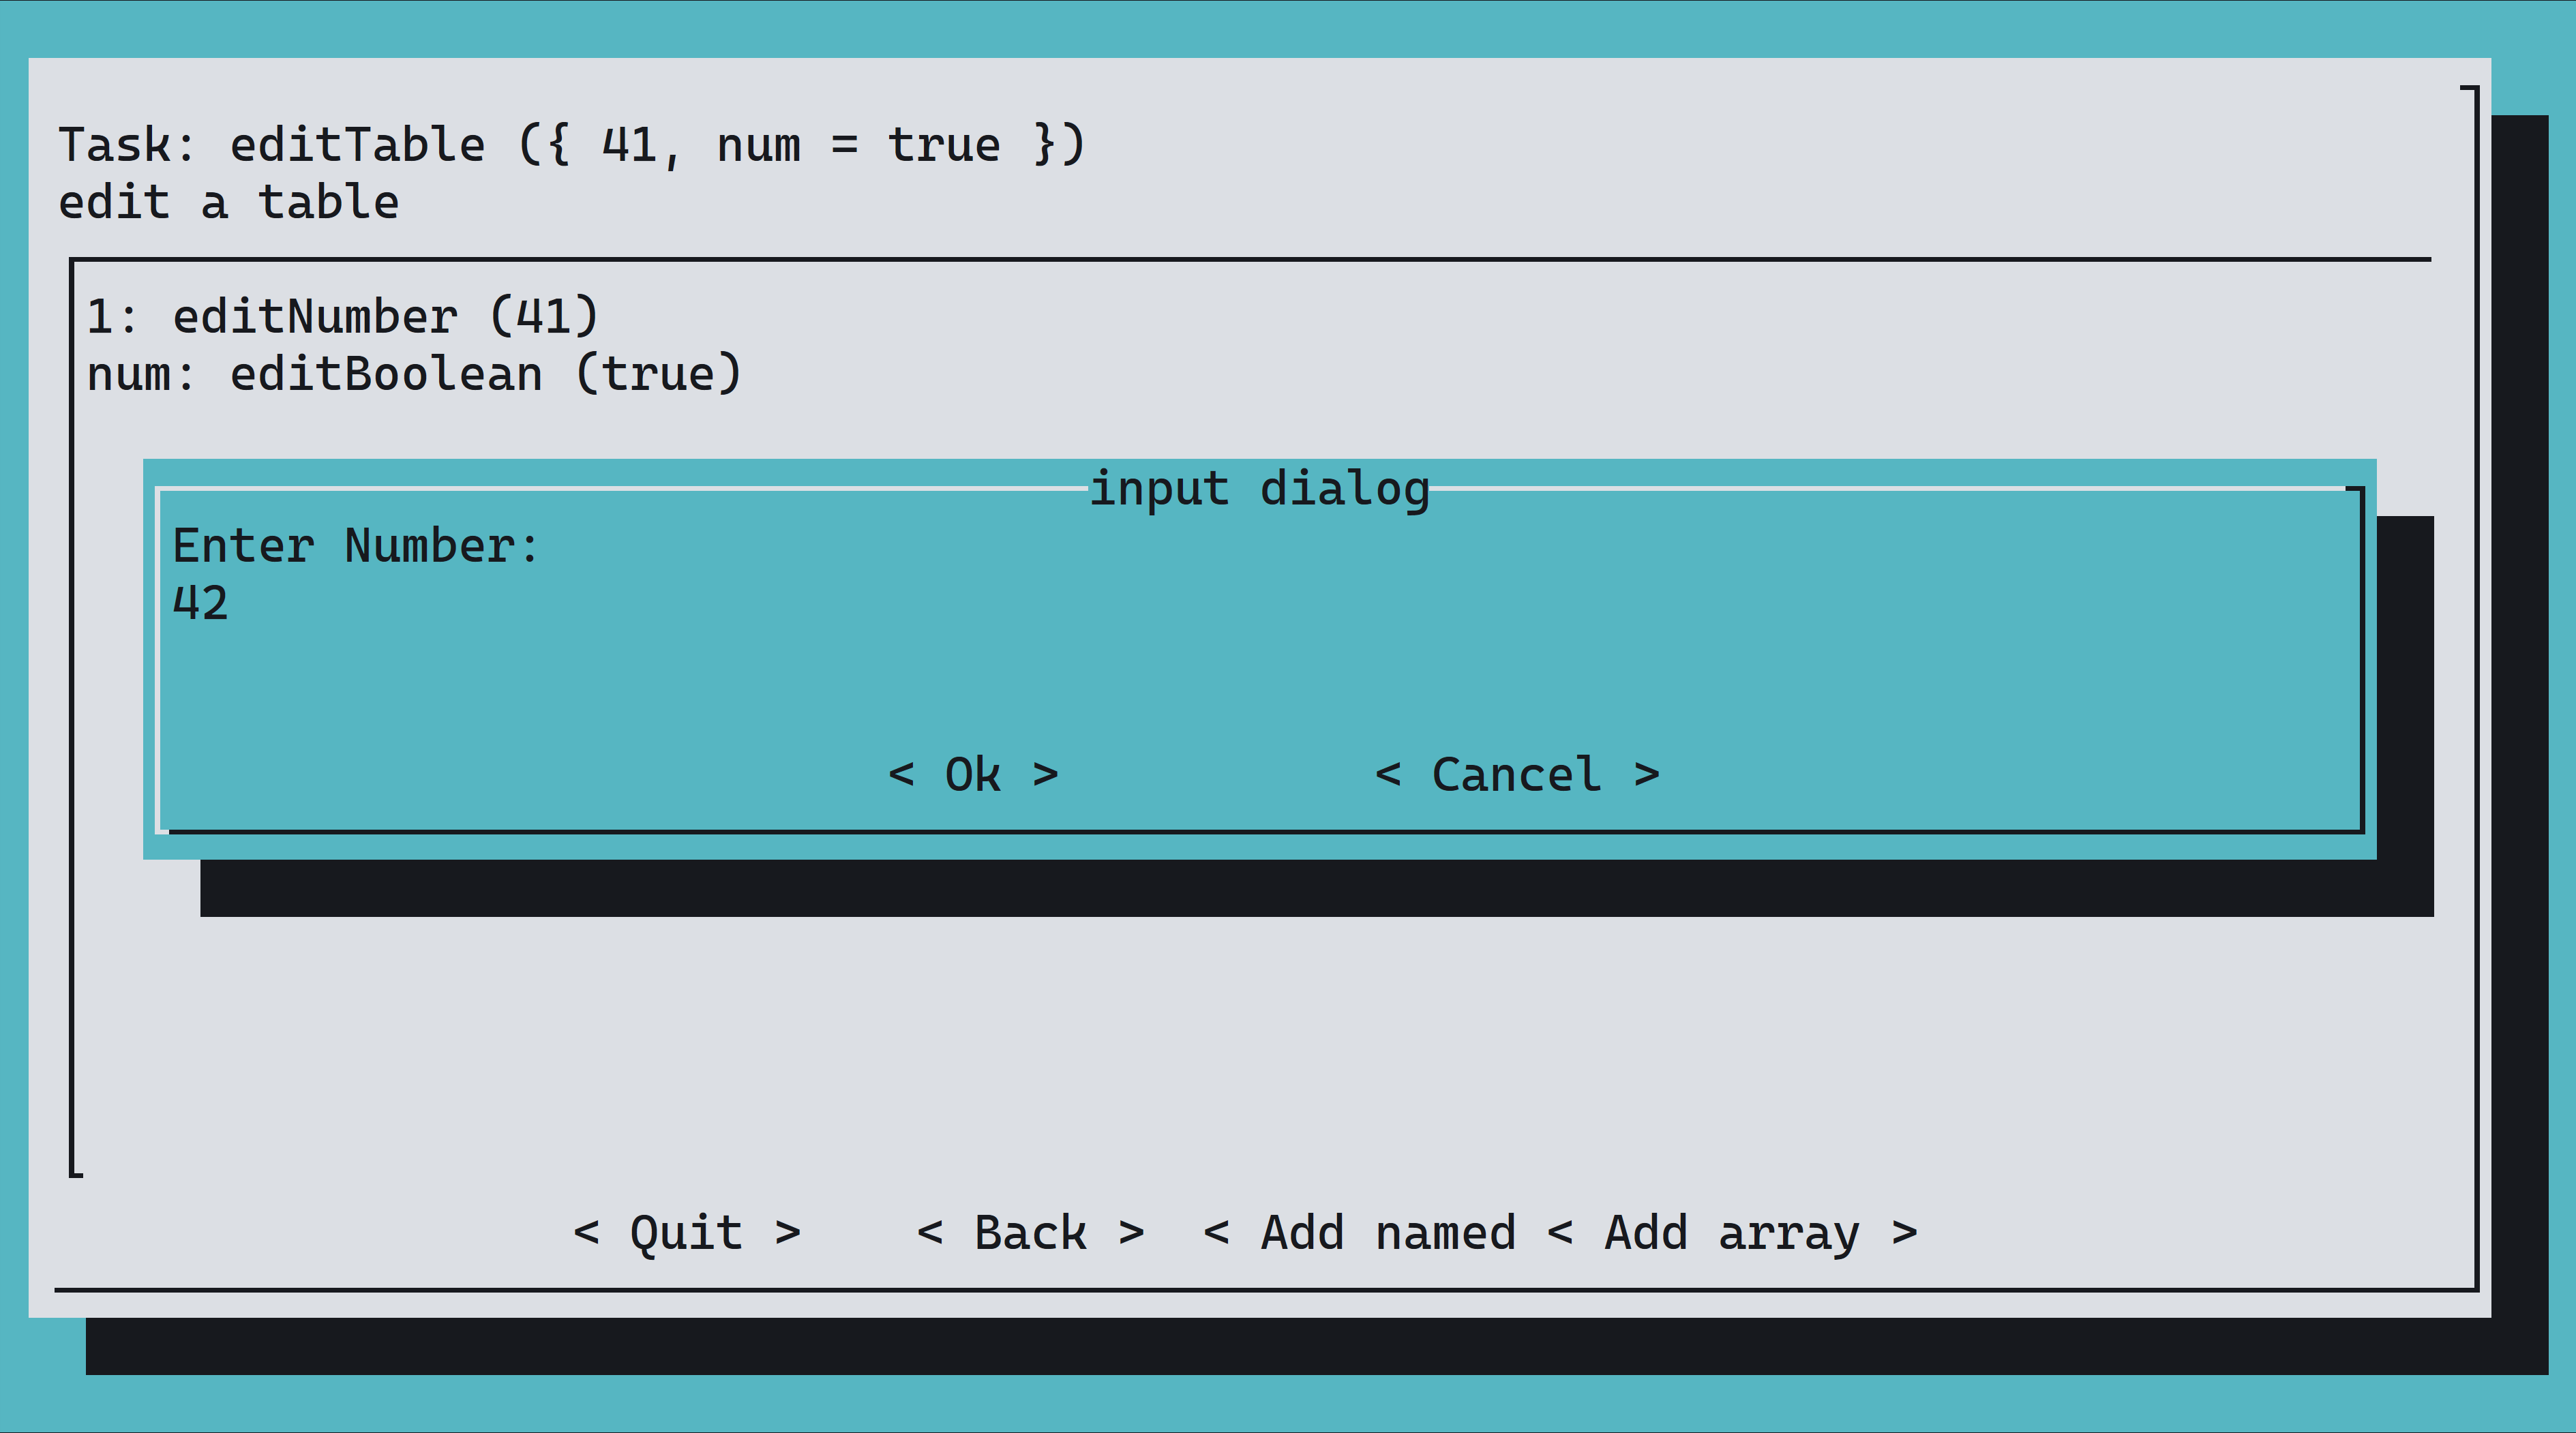
\includegraphics[width=0.8\textwidth]{img/screenshot-ltui.png}
%     \caption{The textual UI showing a table editor in the background with a number input dialog in the foreground.}
%     \label{fig:ltasks_ui}
% \end{figure}
